\section{Aufgabe 3}

\label{sec:Aufgab3}
\lstinputlisting[language=Python, firstline=15, lastline=21]{plots/plot.py}
\paragraph{a)}
Die Mittelwerte $\mu_{P0},\mu_{P1}$ wurden nach den Methoden der VL berechnet in Python wurde dies wie folgt 
implimentiert:
\lstinputlisting[language=Python, firstline=12, lastline=24]{plots/Aufgabe3.py}
Dabei werden in den Zeilen 4 bis 9 nur jeweils die x und y Einträge in arrays geschrieben. Die Mittelwerte 
dieser in ein 2D-array gesetzt ergeben die $\mu_{P0}= \texttt{mup0},\mu_{P1}=\texttt{mup1}$ Mittelwerte. 
Der Mittelwert \texttt{mup001} ist für den Aufgabenteil h.
\paragraph{b)}
Die Kovarianzmatrizen wurden mit einer Numpy Funktion berechnet.
\lstinputlisting[language=Python, firstline=26, lastline=30]{plots/Aufgabe3.py}
Kovarianzmatrix Population 0:
\begin{equation}
\begin{pmatrix}
12.20892862& 8.15840984\\
8.15840984& 6.72286327
\end{pmatrix}
\end{equation}
Kovarianzmatrix Population 1:
\begin{equation}
\begin{pmatrix}
12.35218537 & 7.4107561\\4
 7.41075614 & 5.47731503
\end{pmatrix}
\end{equation}
Kovarianzmatrix Population 0 und 1:
\begin{equation}
\begin{pmatrix}
21.32208007 & 7.94257453\\
 7.94257453 & 6.1025583 
\end{pmatrix}
\end{equation}
Kovarianzmatrix Population 0\_1000:
\begin{equation}
\begin{pmatrix}
12.23612255 & 8.16049883\\
 8.16049883 & 6.75819008
\end{pmatrix}
\end{equation}
Kovarianzmatrix Population 0 und 0\_1000:
\begin{equation}
\begin{pmatrix}
12.21067453 & 8.15842886\\
 8.15842886 & 6.72630542
\end{pmatrix}
\end{equation}
\paragraph{c)} \quad \newline
\lstinputlisting[language=Python, firstline=37, lastline=56]{plots/Aufgabe3.py}
In den Zeilen eins bis drei werden hier nur einmal die Populationen zusammengefasst. Darauf werden 
die Streumatrizen wie aus der VL bestimmt (Zeilen 5-15). Die Lösung für die Fisher Diskriminante 
ist aus der Vl bekannt und wird dann nur noch durch die gegebene Gleichung berechnet (Zeile 17). 
Danach wird diese nur noch normiert. Das selbe (Zeile 17-20) wird für den Aufgabenteil h wiederholt. 
Dann ergibt sich für die Population 0 und 1
\begin{equation}
\vec{\lambda} = \lambda \cdot
\begin{pmatrix}
-0.61886608\\ 
0.78549652
\end{pmatrix}
\end{equation}
und für die Population 0 und 0\_1000:
\begin{equation}
\vec{\lambda} = \lambda \cdot
\begin{pmatrix}
-0.46250292 \\
0.88661776
\end{pmatrix}
\end{equation}
\paragraph{d)}
Zur Berechnung der Projektion wurde folgende Funktion implimentiert:
\lstinputlisting[language=Python, firstline=67, lastline=68]{plots/Aufgabe3.py}
Die Histogramme sind in den Abbildungen \ref{fig:hist01} und \ref{fig:hist001} (Aufgabenteil h) zu sehen.
\begin{figure}
  \centering
  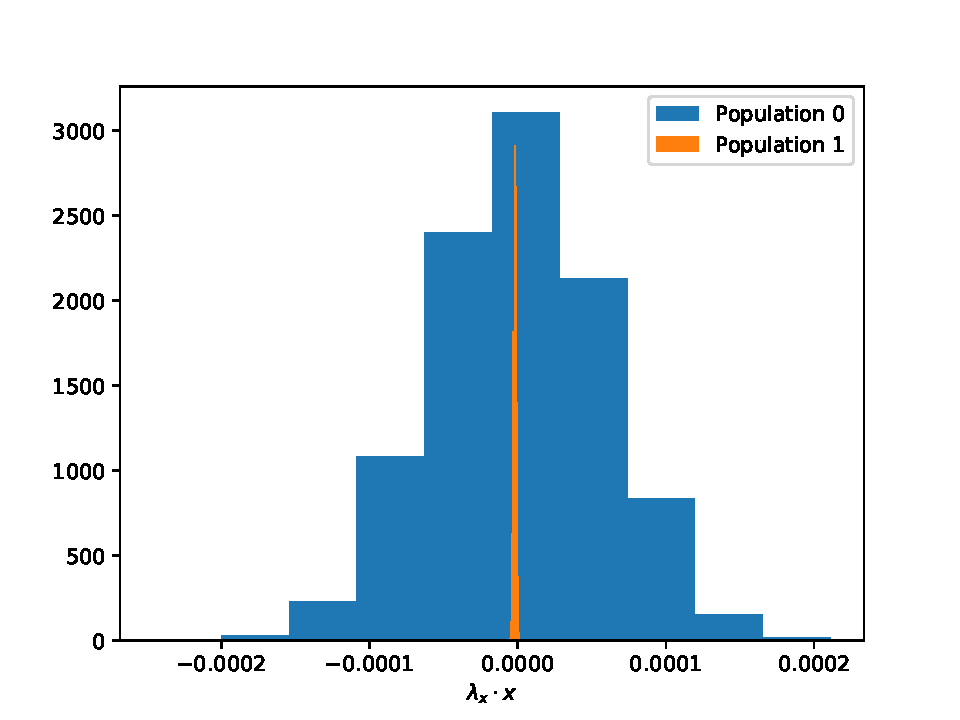
\includegraphics[height = 7cm]{plots/Projektion1dimhist.pdf}
  \caption{Projektion der Populationen 0 und 1.}
  \label{fig:hist01}
\end{figure}
\begin{figure}
  \centering
  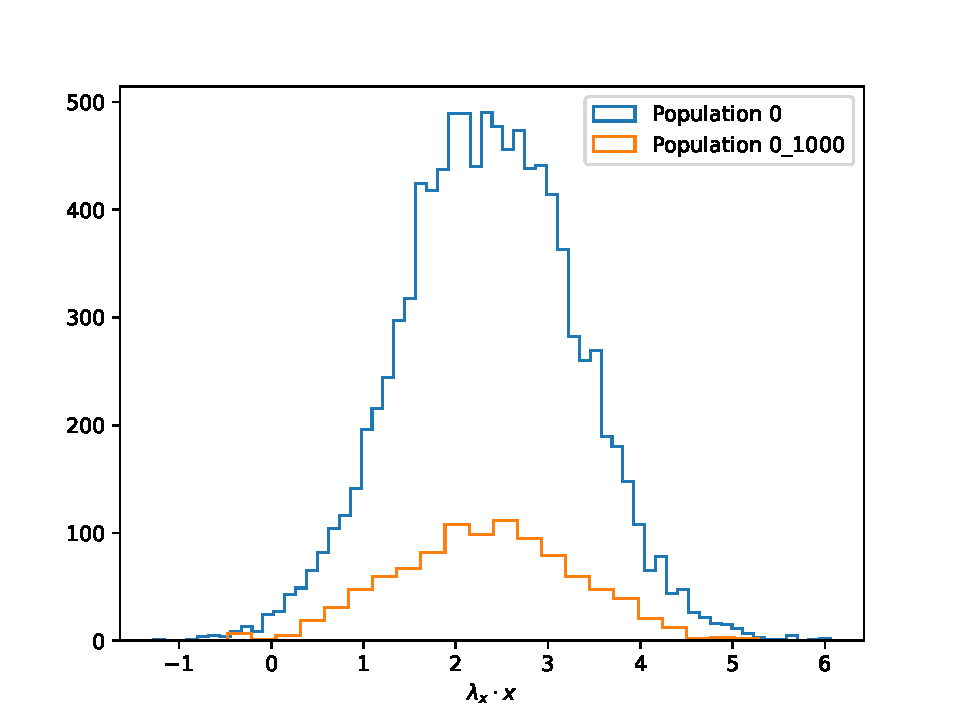
\includegraphics[height = 7cm]{plots/2Projektion1dimhist.pdf}
  \caption{Projektion der Populationen 0 und 0\_1000.}
  \label{fig:hist001}
\end{figure}
\FloatBarrier
\paragraph{e)}
Zur Bestimmung der Reinheit und Effizienz wurde folgende Funktion implimentiert:
\lstinputlisting[language=Python, firstline=86, lastline=102]{plots/Aufgabe3.py}
Die Ergebnisse sind in den Abbildungen \ref{fig:RE1} und \ref{fig:RE2} (AT h) dargestellt. 
Gesuchte $\lambda_{Cut}$ Werte:
\begin{equation}
\lambda_{0\&1} = 2.13667347 \quad \text{und} \quad \lambda_{0\&0\_1} = 5.19070384	\; .
\end{equation}

\begin{figure}
  \centering
  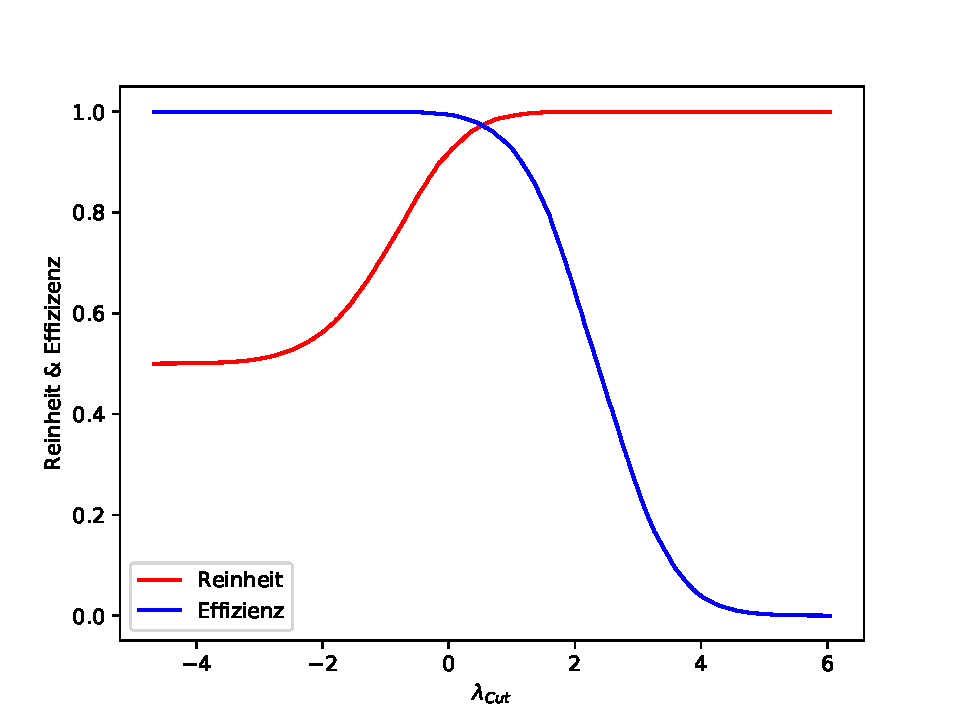
\includegraphics[height = 7cm]{plots/ReinheitEffizienzplot.pdf}
  \caption{Reinheit und Effizienz - Populationen 0 und 1.}
  \label{fig:RE1}
\end{figure}
\begin{figure}
  \centering
  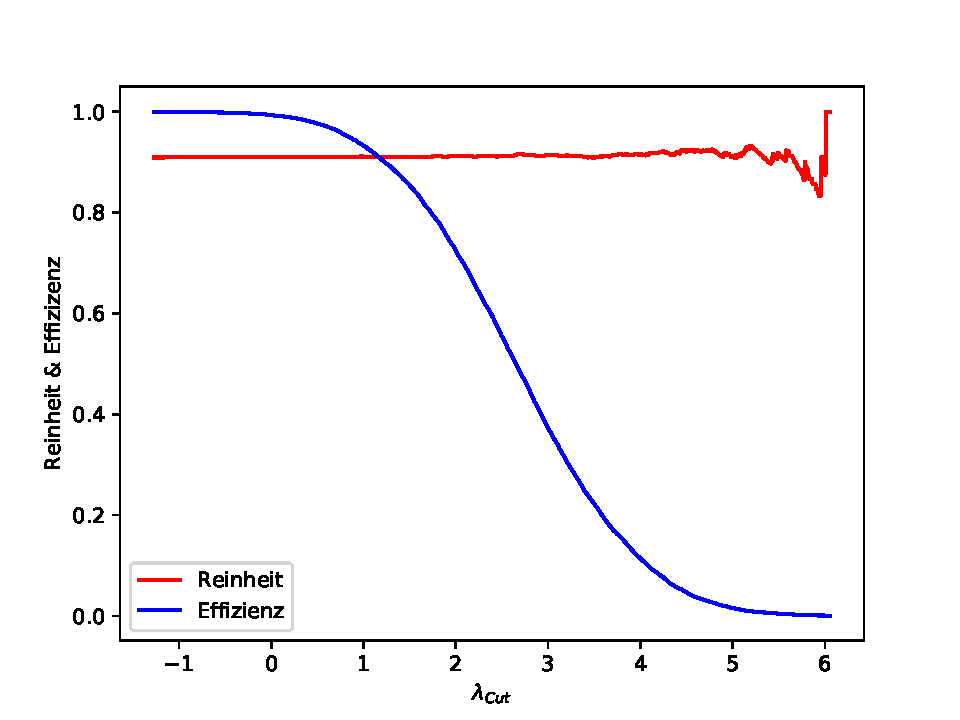
\includegraphics[height = 7cm]{plots/2ReinheitEffizienzplot.pdf}
  \caption{Reinheit und Effizienz - Populationen 0 und 0\_1000.}
  \label{fig:RE2}
\end{figure}
\FloatBarrier
\paragraph{f)}
Zur Berechnung des Signal-Untergrundverhältnisses nach der Trennung wurde folgende Funktion implimentiert. 
\lstinputlisting[language=Python, firstline=125, lastline=134]{plots/Aufgabe3.py}
Die Ergebnisse sind in den Abbildungen \ref{fig:SB1} und \ref{fig:SB1} (AT h) dargestellt. 
Gesuchte $\lambda_{Cut}$ Werte:
\begin{equation}
\lambda_{0\&1} = 0.52587484 \quad \text{und} \quad \lambda_{0\&0\_1} \approx -1.2 \; .	
\end{equation}


\begin{figure}
  \centering
  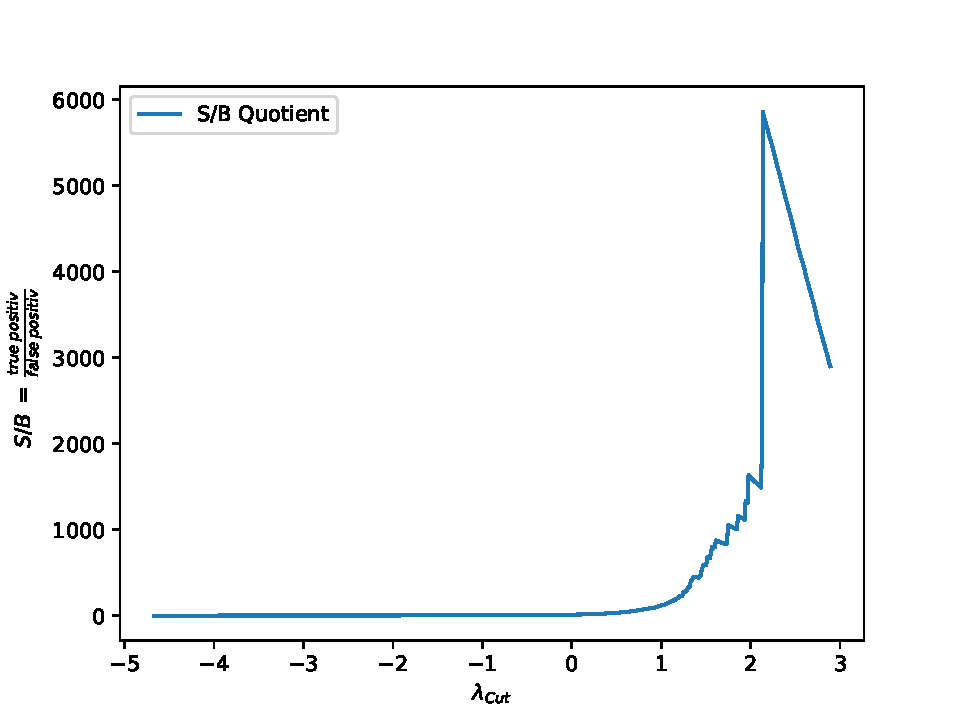
\includegraphics[height = 7cm]{plots/SBRatioplot.pdf}
  \caption{Signal-Untergrundverhältnisses für Populationen 0 und 1.}
  \label{fig:SB1}
\end{figure}
\begin{figure}
  \centering
  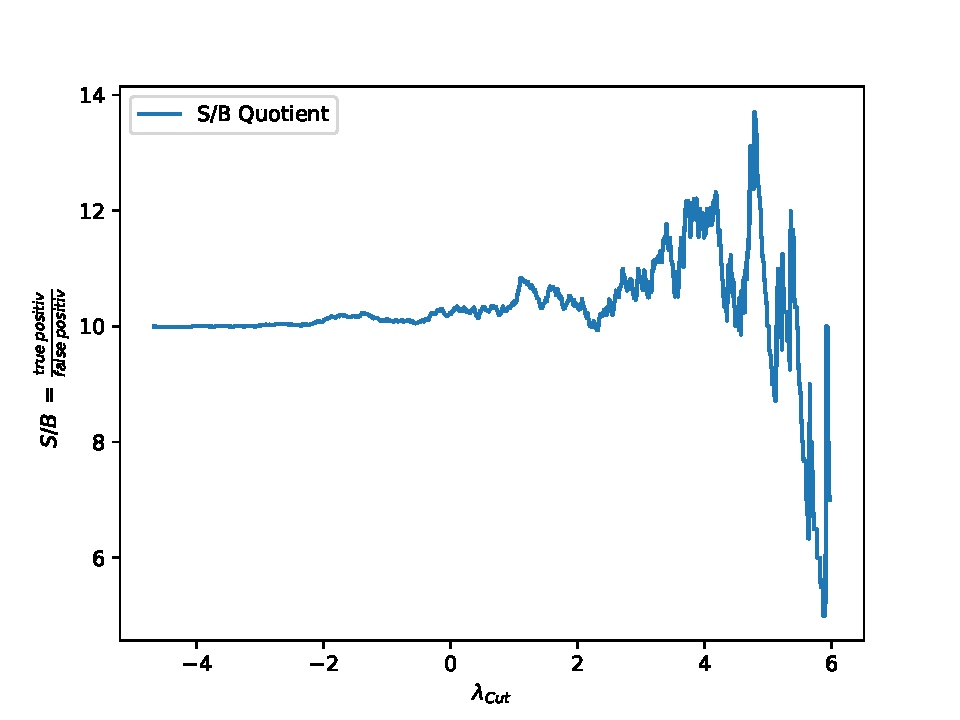
\includegraphics[height = 7cm]{plots/2SBRatioplot.pdf}
  \caption{Signal-Untergrundverhältnisses für Populationen 0 und 0\_1000.}
  \label{fig:SB2}
\end{figure}
\paragraph{g)}
Zur Berechnung der Signifikanz nach der Trennung wurde folgende Funktion implimentiert. 
\lstinputlisting[language=Python, firstline=151, lastline=160]{plots/Aufgabe3.py}
Die Ergebnisse sind in den Abbildungen \ref{fig:S1} und \ref{fig:S2} (AT h) dargestellt. 
\begin{figure}
  \centering
  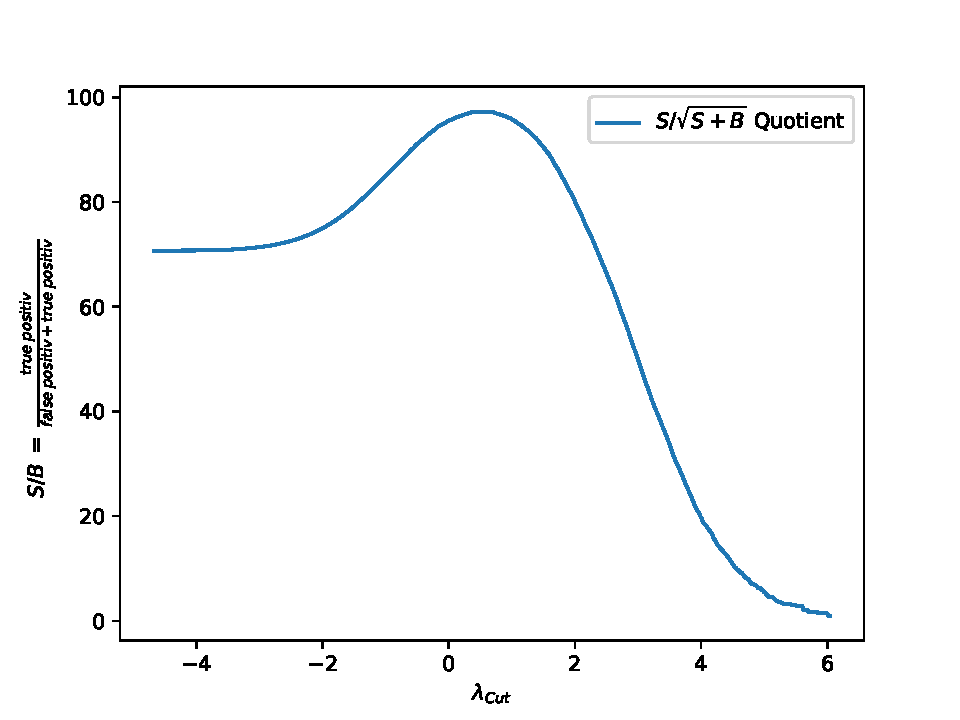
\includegraphics[height = 7cm]{plots/Signifikanzplot.pdf}
  \caption{Signifikanz nach der Trennung Populationen 0 und 1.}
  \label{fig:S1}
\end{figure}
\begin{figure}
  \centering
  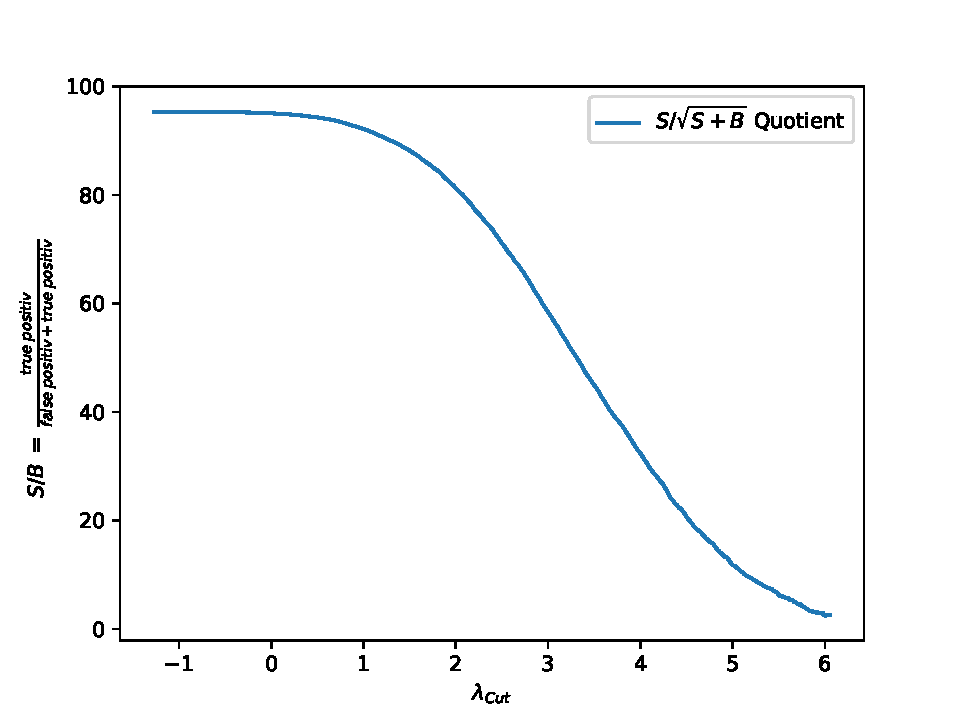
\includegraphics[height = 7cm]{plots/2Signifikanzplot.pdf}
  \caption{Signifikanz nach der Trennung Populationen 0 und 0\_1000.}
  \label{fig:S2}
\end{figure}
\FloatBarrier
\paragraph{d)} siehe oben
